\documentclass[11pt]{td_um}

%------------------------------
\def\version{cor}
%\def\version{eno}
%------------------------------

\makeatletter
%--------------------------------------------------------------------------------

\usepackage[T1]{fontenc}
\usepackage[utf8]{inputenc}
\usepackage[french]{babel}

\usepackage{lmodern}
\usepackage{dsfont}

%\usepackage{qrcode}

\usepackage{eurosym}
\usepackage{diagbox}
\usepackage{enumitem}
%\def\labelitemi{\small \textbullet}
\setlist[itemize,1]{label={\color{gray}\small \textbullet}}
\usepackage{multicol}

\usepackage{graphicx}
\usepackage{float}

\usepackage{array}
\newcolumntype{L}[1]{>{\raggedright\let\newline\\\arraybackslash\hspace{0pt}}m{#1}}
\newcolumntype{C}[1]{>{\centering\let\newline\\\arraybackslash\hspace{0pt}}m{#1}}
\newcolumntype{R}[1]{>{\raggedleft\let\newline\\\arraybackslash\hspace{0pt}}m{#1}}
%----------
%  Version
%-----------

\usepackage{fancyhdr} 
\usepackage{stmaryrd}

%--------
%  Tkz  
%--------
\usepackage{blkarray}
\usepackage[babel=true,kerning=true]{microtype}
\usepackage[caption=false]{subfig}
\usepackage{xcolor,colortbl}
\definecolor{dgreen}{RGB}{0,100,0}
\definecolor{linkcol}{RGB}{0,118,155}
\definecolor{astral}{RGB}{46,116,181}

\usepackage{diagbox,calc,soul,graphicx}

\usepackage{tikz}
\usetikzlibrary{3d,calc,fadings,decorations.pathreplacing,matrix,arrows,decorations.text}
\usetikzlibrary{patterns}
\usetikzlibrary{positioning}
\usetikzlibrary{babel}
\usetikzlibrary{shapes}
\usetikzlibrary{shadings}
\usetikzlibrary{cd}
\usepackage{tikz-3dplot}
\usepackage{pgfplots}
\usepgfplotslibrary{fillbetween}
\pgfplotsset{compat=newest}
\usepgfplotslibrary{external} 
\tikzexternalize[prefix=output_latex/]
\usepgfplotslibrary{fillbetween}
%\graphicspath{{./output-latex/}}


%\usepackage{etex}
%\reserveinserts{28}
%\usepackage{pstricks}
%\usepackage{pst-solides3d}

\usepackage{gnuplot-lua-tikz}

\newcommand\chideux[1]{#1<=0||(#1!=int(#1))?1/0:x<=0?0.0:exp((0.5*#1-1.0)*log(x)-0.5*x-lgamma(0.5*#1)-#1*0.5*log(2))}
\newcommand\gauss[2]{1/(#2*sqrt(2*pi))*exp(-((x-#1)^2)/(2*#2^2))} 
\newcommand\student[1]{gamma(.5*(#1+1))/(sqrt(#1*pi)*gamma(.5*#1))*((1+x^2/#1)^(-.5*(#1+1)))}

% display dices
\usepackage{xparse}\usetikzlibrary{shapes}
\NewDocumentCommand{\drawdie}{O{}m}{%
\begin{tikzpicture}[x=1em,y=1em,radius=0.1,#1,baseline=0.575ex]
		\draw[rounded corners=0.5] (0,0) rectangle (1,1);
	  \ifodd#2
      \fill[] (0.5,0.5) circle;
        \fi
  \ifnum#2>1
      \fill[] (0.2,0.2) circle;
          \fill[] (0.8,0.8) circle;
     \ifnum#2>3
          \fill[] (0.2,0.8) circle;
       \fill[] (0.8,0.2) circle;
           \ifnum#2>5
         \fill[] (0.8,0.5) circle;
       \fill[] (0.2,0.5) circle;
            \ifnum#2>7
           \fill[] (0.5,0.8) circle;
          \fill[] (0.5,0.2) circle;
        \fi
    \fi
      \fi
      \fi
\end{tikzpicture}%
} 
\NewDocumentCommand{\tdrawdie}{O{}m}{%
    \begin{tikzpicture}[x=.6em,y=.6em,radius=0.1,#1,baseline=0.575ex]
		\draw[rounded corners=0.5] (0,0) rectangle (1,1);
	  \ifodd#2
      \fill[] (0.5,0.5) circle;
        \fi
  \ifnum#2>1
      \fill[] (0.2,0.2) circle;
          \fill[] (0.8,0.8) circle;
     \ifnum#2>3
          \fill[] (0.2,0.8) circle;
       \fill[] (0.8,0.2) circle;
           \ifnum#2>5
         \fill[] (0.8,0.5) circle;
       \fill[] (0.2,0.5) circle;
            \ifnum#2>7
           \fill[] (0.5,0.8) circle;
          \fill[] (0.5,0.2) circle;
        \fi
    \fi
      \fi
      \fi
\end{tikzpicture}%
}

\usetikzlibrary{lindenmayersystems}
\pgfdeclarelindenmayersystem{cantor set}{
  \rule{F -> FfF}
  \rule{f -> fff}
}

%------------------
% Math environment
%------------------

\usepackage{latexsym}
\usepackage{amsmath}
\usepackage{amsbsy}
\usepackage{amsfonts}
\usepackage{amssymb}
\usepackage{nicefrac}
\usepackage{amscd}
\usepackage{amsthm}
\usepackage{mathtools}

\newtheoremstyle{definitionSs}{\topsep}{\topsep}%
     {}%         Body font
     {}%         Indent amount (empty = no indent, \parindent = para indent)
     {\sffamily\bfseries}% Thm head font
     {.}%        Punctuation after thm head
     { }%     Space after thm head (\newline = linebreak)
     {\thmname{#1}\thmnumber{~#2}\thmnote{~#3}}%         Thm head spec

\newtheoremstyle{plainSs}{\topsep}{\topsep}%
     {\itshape}%         Body font
     {}%         Indent amount (empty = no indent, \parindent = para indent)
     {\sffamily\bfseries}% Thm head font
     {.}%        Punctuation after thm head
     { }%     Space after thm head (\newline = linebreak)
     {\thmname{#1}\thmnumber{~#2}\thmnote{~#3}}%         Thm head spec

\theoremstyle{definitionSs}
\newtheorem{remark}{Remarque}[section]
\newtheorem*{remark*}{Remarque}
\newtheorem{example}{Exemple}[section]


%\usepackage[framemethod=tikz]{mdframed}
\usepackage[]{mdframed}

\newmdtheoremenv[
hidealllines=true,
leftline=true,
skipabove=0pt,
innertopmargin=-5pt,
innerbottommargin=2pt,
linewidth=4pt,
linecolor=gray!90,
innerrightmargin=0pt,
]{definition}{Définition}[section]

\newmdtheoremenv[
hidealllines=true,
leftline=true,
skipabove=0pt,
innertopmargin=-5pt,
innerbottommargin=2pt,
linewidth=4pt,
linecolor=gray!40,
innerrightmargin=0pt,
]{lemme}{Lemme}[section]

\newmdtheoremenv[
hidealllines=true,
leftline=true,
skipabove=0pt,
innertopmargin=-5pt,
innerbottommargin=2pt,
linewidth=4pt,
linecolor=gray!40,
innerrightmargin=0pt,
]{proposition}{Proposition}[section]

\newmdtheoremenv[
hidealllines=true,
leftline=true,
skipabove=0pt,
innertopmargin=-5pt,
innerbottommargin=2pt,
linewidth=4pt,
linecolor=gray!40,
innerrightmargin=0pt,
]{corollaire}{Corollaire}[section]

\newmdtheoremenv[
hidealllines=true,
leftline=true,
skipabove=0pt,
innertopmargin=-5pt,
innerbottommargin=2pt,
linewidth=4pt,
linecolor=gray!90,
innerrightmargin=0pt,
]{propdef}{Définition - Proposition}[section]

\newmdtheoremenv[
hidealllines=true,
leftline=true,
skipabove=0pt,
innertopmargin=-5pt,
innerbottommargin=2pt,
linewidth=4pt,
linecolor=gray!100,
innerrightmargin=0pt,
]{theorem}{Théorème}[section]

%---------------
% Mise en page
%--------------

\setlength{\parindent}{0pt}

\renewcommand*{\descriptionlabel}[1]{\hspace\labelsep{\sffamily #1}}
\providecommand{\defemph}[1]{{\sffamily\bfseries\color{astral}#1}}
\renewcommand{\emph}[1]{{\sffamily #1}}

%\usepackage{titlesec, blindtext, color}
%\newcommand{\hsp}{\hspace{20pt}}
%\titleformat{\chapter}[hang]{\sffamily\Huge\bfseries}{\thechapter\hsp\textcolor{gray75}{|}\hsp}{0pt}{\Huge\bfseries}
\usepackage{sectsty}
\allsectionsfont{\color{astral}\normalfont\sffamily\bfseries}

\usepackage[subfigure]{tocloft}
\renewcommand{\cfttoctitlefont}{\sffamily\bfseries\Huge\color{astral}}
\renewcommand{\cftchapfont}{\sffamily\bfseries\color{astral}}
\renewcommand{\cftsecfont}{\sffamily\bfseries}
\renewcommand{\cftsubsecfont}{\sffamily}
\usepackage{hyperref}
\hypersetup{linktocpage, colorlinks=true, linkcolor=gray, urlcolor=linkcol, citecolor=gray}


%----------------
% Some commands
%----------------

\makeatletter
\newcommand\RedeclareMathOperator{%
  \@ifstar{\def\rmo@s{m}\rmo@redeclare}{\def\rmo@s{o}\rmo@redeclare}%
}
% this is taken from \renew@command
\newcommand\rmo@redeclare[2]{%
  \begingroup \escapechar\m@ne\xdef\@gtempa{{\string#1}}\endgroup
  \expandafter\@ifundefined\@gtempa
     {\@latex@error{\noexpand#1undefined}\@ehc}%
     \relax
  \expandafter\rmo@declmathop\rmo@s{#1}{#2}}
% This is just \@declmathop without \@ifdefinable
\newcommand\rmo@declmathop[3]{%
  \DeclareRobustCommand{#2}{\qopname\newmcodes@#1{#3}}%
}
\@onlypreamble\RedeclareMathOperator
\makeatother

\newcommand{\skipline}{\vspace{\baselineskip}}
\newcommand{\noi}{\noindent}


%----- Raccourci proba ------------------
\newcommand{\Om}{\Omega}
\newcommand{\Tribu}{\cF}
\newcommand{\Tribubis}{\cG}
\newcommand{\Partie}{\cE}
\newcommand{\Proba}{\bbP}
\newcommand{\Espe}{\bbE}
\newcommand{\OF}{(\Om,\Tribu)}
\newcommand{\RBR}{\big(\bbR,\cB(\bbR)\big)}
\newcommand{\OFP}{(\Om,\Tribu,\Proba)}
\newcommand{\POm}{\cP(\Om)}
\newcommand{\Leb}{\lambda}
%----- Lettres -------------------------
\newcommand{\bbC}{\mathbb{C}}
\newcommand{\bbE}{\mathbb{E}}
\newcommand{\bbF}{\mathbb{F}}
\newcommand{\bbG}{\mathbb{G}}
\newcommand{\bbK}{\mathbb{K}}
\newcommand{\bbL}{\mathbb{L}}
\newcommand{\bbN}{\mathbb{N}}
\newcommand{\bbP}{\mathbb{P}}
\newcommand{\bbQ}{\mathbb{Q}}
\newcommand{\bbR}{\mathbb{R}}
\newcommand{\bbS}{\mathbb{S}}
\newcommand{\bbT}{\mathbb{T}}
\newcommand{\bbU}{\mathbb{U}}
\newcommand{\bbZ}{\mathbb{Z}}

\newcommand{\bfC}{\mathbf{C}}
\newcommand{\bfE}{\mathbf{E}}
\newcommand{\bfL}{\mathbf{L}}
\newcommand{\bfN}{\mathbf{N}}
\newcommand{\bfP}{\mathbf{P}}
\newcommand{\bfQ}{\mathbf{Q}}
\newcommand{\bfR}{\mathbf{R}}
\newcommand{\bfZ}{\mathbf{Z}}

\newcommand{\calA}{\mathcal{A}}
\newcommand{\calB}{\mathcal{B}}
\newcommand{\calC}{\mathcal{C}}
\newcommand{\calE}{\mathcal{E}}
\newcommand{\calF}{\mathcal{F}}
\newcommand{\calG}{\mathcal{G}}
\newcommand{\calJ}{\mathcal{J}}
\newcommand{\calL}{\mathcal{L}}
\newcommand{\calM}{\mathcal{M}}
\newcommand{\calN}{\mathcal{N}}
\newcommand{\calO}{\mathcal{O}}
\newcommand{\calP}{\mathcal{P}}
\newcommand{\calS}{\mathcal{S}}
\newcommand{\calT}{\mathcal{T}}
\newcommand{\calV}{\mathcal{V}}
\newcommand{\calX}{\mathcal{X}}

\newcommand{\fA}{\mathfrak{A}}
\newcommand{\fB}{\mathfrak{B}}
\newcommand{\fF}{\mathfrak{F}}

% la droite réelle achevée
\newcommand{\barR}{\overline{\mathbb{R}}}

%
%------------------------------- Majuscules calligraphiques
\renewcommand{\geq}{\geqslant}
\renewcommand{\ge}{\geqslant}
\renewcommand{\leq}{\leqslant}
\renewcommand{\le}{\leqslant}
%
\usepackage{mathrsfs}
\newcommand{\scrL}{\mathscr{L}}
\newcommand{\scrF}{\mathscr{F}}
\newcommand{\scrM}{\mathscr{M}}
\newcommand{\scrD}{\mathscr{D}}
\newcommand{\scrE}{\mathscr{E}}
\newcommand{\scrA}{\mathscr{A}}
\newcommand{\scrB}{\mathscr{B}}
\newcommand{\scrC}{\mathscr{C}}
\newcommand{\scrI}{\mathscr{I}}
\newcommand{\scrJ}{\mathscr{J}}
\newcommand{\scrK}{\mathscr{K}}
\newcommand{\scrS}{\mathscr{S}}
\newcommand{\scrO}{\mathscr{O}}
\newcommand{\scrP}{\mathscr{P}}
\newcommand{\scrR}{\mathscr{R}}
\newcommand{\scrT}{\mathscr{T}}
\newcommand{\scrZ}{\mathscr{Z}}
%
\newcommand{\vois}{\mathscr{V}}
\newcommand{\ouv}{\mathscr{O}}
\newcommand{\ferm}{\mathscr{F}}

%
%------------------------------- Intervalles
%
\newcommand{\oo}[1]{\mathopen{]}#1\mathclose{[}}
\newcommand{\fo}[1]{\mathopen{[}#1\mathclose{[}}
\newcommand{\of}[1]{\mathopen{]}#1\mathclose{]}}
\newcommand{\ff}[1]{\mathopen{[}#1\mathclose{]}}
\newcommand{\lbb}{[\![}
\newcommand{\rbb}{]\!]}

%
\newcommand{\ex}{e}
\newcommand{\ind}{\mathrm{Ind}}
\newcommand{\spt}{\mathrm{Spt}}
\newcommand{\pd}{\frac{\pi}{2}}
\newcommand{\E}{\mathrm{E}}
\newcommand{\diff}{\mathrm{Diff}}
\newcommand{\diam}{\mathrm{diam}}
\newcommand{\comp}[1]{#1^\mathrm{c}}
\newcommand{\vvv}{|\!|\!|}
\newcommand{\dd}[2]{\frac{\partial #1}{\partial #2}}
%
%----- chapeaux, tildes -------------------------
\newcommand{\wb}[1]{\overline{#1}}
\newcommand{\wh}[1]{\widehat{#1}}
\newcommand{\wt}[1]{\widetilde{#1}}

%----- ccouleurs -------------------------
\newcommand{\rose}[1]{\textcolor{magenta}{#1}}

%----- Maths -----------------------
\newcommand {\expl}[2]{\mathrm{e}^{-\Lambda(#1,#2)}}
\newcommand {\expla}[2]{\mathrm{e}^{-\alpha #2-\Lambda(#1,#2)}}
\newcommand {\Li}[1]{[ #1 ]}
%\newcommand{\1}{\mathbbm{1}}
\newcommand {\tstar}[1]{t^{*}(#1)}
\DeclareMathOperator{\aire}{Aire}
\providecommand{\gf}{g\circ f}
\providecommand{\R}{\ensuremath \mathbb{R}}
\providecommand{\C}{\ensuremath \mathbb{C}}
\providecommand{\reg}[1]{\mathcal{C}^{#1}}
\providecommand{\N}{\mathbb{N}}
\providecommand{\M}{\mathcal{M}}
\providecommand{\Q}{\mathbb{Q}}
\renewcommand{\L}{\mathcal{L}}
\providecommand{\D}{\mathcal{D}}
\providecommand{\Cc}{\mathcal{C}}
\providecommand{\F}{\mathcal{F}}
\providecommand{\Ee}{\mathcal{E}}
\providecommand{\G}{\mathcal{G}}
\providecommand{\Z}{\mathbb{Z}}
\providecommand{\x}{\ensuremath\boldsymbol{x}}
\providecommand{\y}{\ensuremath\boldsymbol{y}}
\providecommand{\1}{\mathds{1}}
\providecommand{\p}{\partial}
\providecommand{\Pp}{\mathcal{P}}
\providecommand{\P}{\mathbb{P}}
\providecommand{\E}{\mathbb{E}}
\providecommand{\U}{\mathcal{U}}
\providecommand{\V}{\mathcal{V}}
\providecommand{\ie}{\textit{i.e. }}
\renewcommand{\P}{\mathbb{P}}
\renewcommand{\S}{\mathcal{S}}
\providecommand{\E}{\mathbb{E}}
\providecommand{\one}{\mathds{1}}
\DeclareMathOperator{\card}{Card}
\DeclareMathOperator{\vol}{Vol}
\DeclareMathOperator{\var}{Var}
\DeclareMathOperator{\vect}{\mathsf{Vect}}
\DeclareMathOperator{\med}{median}
\DeclareMathOperator{\hess}{Hess}
\DeclareMathOperator{\jac}{Jac}
\DeclareMathOperator{\cov}{cov}
\DeclareMathOperator{\diag}{\mathsf{Diag}}
\DeclareMathOperator{\im}{\mathsf{Im}}
\DeclareRobustCommand{\re}{\mathsf{Re}}
\RedeclareMathOperator{\ker}{\mathsf{Ker}}
\RedeclareMathOperator{\det}{\mathsf{det}}
\DeclareMathOperator{\rank}{\mathsf{rank}}
\DeclareMathOperator{\tr}{\mathsf{tr}}
\DeclareMathOperator{\id}{\mathsf{Id}}
\DeclareMathOperator{\can}{\mathsf{can}}
\DeclareMathOperator{\com}{\mathsf{com}}
\DeclareMathOperator*{\argmax}{Argmax}
\providecommand{\B}{\mathsf{B}}

\providecommand{\ncd}{\norm{\cdot}}
\providecommand{\norm}[1]{\left\lVert#1\right\rVert}
\providecommand{\bnorm}[1]{\bigg\lVert#1\bigg\rVert}
\providecommand{\snorm}[1]{\lVert#1\rVert}

\newcommand{\tnorm}[1]{{\left\vert\kern-0.25ex\left\vert\kern-0.25ex\left\vert #1 
    \right\vert\kern-0.25ex\right\vert\kern-0.25ex\right\vert}}

\providecommand{\abs}[1]{\left\lvert#1\right\rvert}
\providecommand{\sabs}[1]{\lvert#1\rvert}
\providecommand{\Babs}[1]{\bigg\lvert#1\bigg\rvert}
\providecommand{\babs}[1]{\bigg\lvert#1\bigg\rvert}

\providecommand{\prscd}{\prs{\cdot,\cdot}}
\providecommand{\prs}[1]{\left\langle #1\right\rangle}
\providecommand{\sprs}[1]{\langle #1\rangle}
\providecommand{\bprs}[1]{\bigg\langle #1\bigg\rangle}

\providecommand{\rev}{$\R$ espace vectoriel}

\providecommand{\dpar}[2]{\frac{\partial #1}{\partial #2}}

\newcommand\rst[2]{{#1}_{\restriction_{#2}}}


% Multiversioning 


\usepackage{ifthen}

\newcommand{\pl}[2]{%
	\ifthenelse{\equal{\version}{poly}}{#1}{}%
	\ifthenelse{\equal{\version}{print}}{#2}{}%
}
\newcommand{\plprof}[1]{\ifthenelse{\equal{\version}{print}}{#1}{}}
\newcommand{\sld}[1]{\ifthenelse{\equal{\version}{slide}}{#1}{}}

\newcommand{\eno}[1]{%
	\ifthenelse{\equal{\version}{eno}}{#1}{}%
}
\newcommand{\cor}[1]{%
        \ifthenelse{\equal{\version}{cor}}{
\medskip 

{\small \color{gray} #1}

\medskip 
}{}
}

\mdfdefinestyle{response}{
	leftmargin=.01\textwidth,
	rightmargin=.01\textwidth,
	linewidth=1pt
	hidealllines=false,
	leftline=true,
	rightline=true,topline=true,bottomline=true,
        skipabove=\baselineskip,%0pt,
	%innertopmargin=-5pt,
	%innerbottommargin=2pt,
	linecolor=gray,
	innerrightmargin=0pt,
	}
\providecommand{\rep}[1]{$ $ \newline \begin{mdframed}[style=response] \vspace*{#1} \end{mdframed}}

% generate breakable white space allowing students to write notes.
\newcommand*{\DivideLengths}[2]{%
  \strip@pt\dimexpr\number\numexpr\number\dimexpr#1\relax*65536/\number\dimexpr#2\relax\relax sp\relax
}

\usepackage{xparse}
\ExplSyntaxOn
\NewDocumentCommand\manyvspace { m }
 {
  \par
  \int_step_inline:nn{#1}{\phantom{.}\vspace*{1em}\goodbreak}
 }
\ExplSyntaxOff 

%\providecommand{\rep}[1]{$ $

    %\begin{mdframed}[style=response]  
	%\vspace*{\DivideLengths{#1}{3cm}cm}
	%\pagebreak[1]	
	%\vspace*{\DivideLengths{#1}{3cm}cm}
	%\pagebreak[1]		
	%\vspace*{\DivideLengths{#1}{3cm}cm}
    %\end{mdframed}%
%}
\providecommand{\repcom}[1]{\begin{mdframed}[style=response] #1 \end{mdframed}}
\providecommand{\comexo}[1]{\bigskip {\color{gray}#1}}
\providecommand{\blanc}[1]{\vspace*{#1}}
\providecommand{\myeq}[1]{\mathrel{\overset{\makebox[0pt]{\mbox{\normalfont\tiny #1}}}{=}}}
\def\redspace{\sld{\setlength{\belowdisplayskip}{0pt} \setlength{\belowdisplayshortskip}{0pt}\setlength{\abovedisplayskip}{0pt}\setlength{\abovedisplayshortskip}{0pt}}}
%------------------------------------------------------------------------------
%\DeclareUnicodeCharacter{00A0}{~}

\pdfstringdefDisableCommands{%
    %\renewcommand*{\bm}[1]{#1}%
    \renewcommand*{\R}{R}%
    % any other necessary redefinitions 
}
\makeatother




\newcommand{\va}{variable aléatoire\xspace} 
\newcommand{\vas}{variables aléatoires\xspace}
\newcommand{\evs}{événements\xspace}
\newcommand{\ev}{événement\xspace}
\newcommand{\fdr}{fonction de répartition\xspace} 
\usepackage{xspace} % gestion des espaces apres les macros

\title{TD 4 - Marche Aléatoire}

\begin{document}

\maketitle


\bigskip

\bigskip


\begin{exo}{} % loi de S_n
Soit $(S_n)$ une marche aéatoire issue de $S_0=0$. 
\begin{enumerate}
    \item  Calculer la loi de $S_1$, $S_2$ et $S_3$.
%--------------------------------------------
        \cor{
            \begin{itemize}
                \item     $S_1=X_1$ prend les valeurs $-1$ et $1$ avec probabilité $1/2$.
                \item    $S_2=X_1+X_2$ prend les valeurs $-2$ avec proba $1/4$, $0$ avec proba $1/2$, $2$ avec proba $1/4$.
                \item  $S_3=X_1+X_2+X_3$ prend les valeurs $-3$ avec proba $1/8$, $-1$ avec proba $3/8$, $1$ avec proba $3/8$, $3$ avec proba $1/8$
            \end{itemize}
        }
%--------------------------------------------
    \item Calculer la loi de $(n+S_n)/2$  pour tout $n$.
%--------------------------------------------
        \cor{
            Posons $Y_k = (X_k+1)/2$. Alors on a que les v.a. $Y_k$ sont iid de loi $B(1/2)$.
            Ainsi $(S_n+n)/2=\sum_{k=1}^n(X_k+1)/2=\sum_{k=1}^nY_k$ suit la loi $B(n,1/2)$.
        }
%--------------------------------------------
    \item En déduire la loi de $S_n$ pour tout $n$.
%--------------------------------------------
        \cor{
            $S_n=2((S_n+n)/2)-n$ donc la loi de $S_n$ est une loi binomiale décalée : $S_n$ prend les valeurs $2k-n$ pour $0\leq k\leq n$ et $\bbP(S_n=2k-n)=\binom{n}{k} 2^{-n}$.
        }
%--------------------------------------------
\end{enumerate}
\end{exo}




\begin{exo}{} % Scrutin
Cent personnes font la queue à un guichet de cinéma. La place coûte $5$~\euro{} et 60 personnes ont un billet de $5$~\euro{} tandis que les 40 autres ont des billets de $10$~\euro{}. Combien faut-il prévoir de billets de $5$~\euro{} en caisse pour que toutes les spectatrices et les spectateurs soient servis dans leur ordre d'arrivée avec une probabilité d'au moins $95\%$?
%--------------------------------------------
\cor{
On modélise l'argent en caisse par les chemins d'une marche aléatoire. Mais attention, ici la loi des incréments n'est pas i.i.d.: c'est un tirage sans remise dans une population de 60 $+1$ contre 40 $-1$. Soit donc $S_n$ le nombre de billets de $5$\euro{} en caisse après le passage de la $n$-ème personne. On a $S_0=x$ inconnue et $S_{100}=60-40+x=20+x$ puisque $60$ personnes ont payé avec un billet de $5$\euro{} et qu'il a fallu rendre la monnaie au $40$ personnes payant avec un billet de $10$\euro{}. 

Un tirage où toutes les spectatrices et les spectateurs sont servis correspond à un chemin de $(0,x)$ à $(100,20+x)$ qui ne touche pas $-1$. Dénombrons ces chemins. Le nombre de chemins de  $(0,x)$ à $(100,20+x)$ qui ne touchent pas $-1$ est égal
\begin{itemize}
\item au nombre de chemins de  $(0,x+1)$ à $(100,20+x+1)$ qui ne touchent pas $0$, par translation verticale;
\item au nombre total de chemins de $(0,x+1)$ à $(100,20+x+1)$ moins le nombre de chemins de $(0,x+1)$ à $(100,20+x+1)$ qui passent par $0$;
\item au nombre total de chemins de $(0,x+1)$ à $(100,20+x+1)$ moins le nombre total de chemins de $(0,x+1)$ à $(100,-(21+x))$ par le principe de réflexion.
\end{itemize}
La probabilité de satisfaire tout le monde est alors le nombre de chemins ci-dessus divisé par le nombre total de chemins de  $(0,x)$ à $(100,20+x)$ puisqu'ils sont tous équiprobables (cela revient à choisir une permutation de l'ordre de passage). On obtient ainsi que cette probabilité vaut
\begin{align*}
p&=\frac{\binom{100}{60}-\binom{100}{50+11+x}}{\binom{100}{60}}\\
&=1-\frac{60!40!100!}{100!(61+x)!(39-x)!}\\
&=1-\frac{60!}{(61+x)!}\frac{40!}{(39-x)!}.
\end{align*}

Les valeurs de $p$ pour $x$ entre $0$ et $5$ sont
\begin{center}
\begin{tabular}{l|rrrrrr}
\hline
$x$&0&1&2&3&4&5\\
\hline
$p$&$0.3443$&$0.5875$&$0.7512$&$0.8562$&$0.9203$&$0.9578$\\
\hline
\end{tabular}
\end{center}
%
On constate qu'à partir de $x=5$ cette probabilité dépasse $95\%$.
}
%--------------------------------------------
\end{exo}


\begin{exo}{} %variantes de la réflexion
Si $a$ et $b$ sont deux entiers strictement positifs, montrer qu'il y a autant de chemins de $0$ à $a+b$ que de chemins de même longueur de $0$ à $a-b$ passant par $a$.
%-----------------------
\cor{
Le nombre de chemins de $(0,0)$ à $(n,a+b)$  est égal
\begin{itemize}
\item au nombre de chemins de $(0,-a)$ à $(n,b)$ par translation verticale;
\item au nombre de chemins de $(0,-a)$ à $(n,-b)$ passant par $0$ par le principe de réflexion, puisque $a$ et $b$ ont le même signe;
\item au nombre de chemins de $(0,0)$ à $(n,a-b)$ passant par $a$ par translation verticale.
\end{itemize}
}
%-----------------------
\end{exo}


\begin{exo}{} %Jeux
 Une joueuse dispose de $10$~\euro{} pour jouer à une machine à sous. A chaque partie, elle met $1$~\euro{} dans la machine et celle-ci rend $2$~\euro{} ou rien avec équiprobabilité.
 \begin{enumerate}
     \item  Modéliser la fortune de la  joueuse par une marche aéatoire.
%--------------------------------------------
         \cor{
             Modélisons la fortune de la  joueuse par une marche aéatoire. Soit $S_n$ la fortune de la joueuse après le $n$-ème jeu. On sait que $S_0=10$, et pour tout $n\geq 0$, $S_{n+1}=S_n+X_{n+1}$ où $X_{n}$ représente le gain du $n$-ème jeu. Les variables aléatoires $X_k$ sont indépendantes, de même loi donnée par 
             \begin{align*}
                 \bbP(X_1=-1+2)=\bbP(X_1=-1+0)=\frac{1}{2}.
             \end{align*}
             Donc $(S_n)_{n\geq 0}$ est bien une marche aléatoire simple symétrique.
         }
%--------------------------------------------
         Soit $N$ le nombre de parties jouées jusqu'à la ruine de la joueuse.
     \item  Quelle est la parité de $N$? Quelle valeur minimale peut-il prendre? 
%--------------------------------------------
         \cor{
             Comme la richesse initiale est paire, la joueuse ne peut être ruinée qu'en un nombre pair de parties. De plus, comme elle perd au maximum $1$ à chaque partie, elle ne peut pas être ruinée avant la fin de la $10$-ème partie.
         }
%--------------------------------------------
     \item  Calculer la loi de $N$.
%--------------------------------------------
         \cor{
             Calculons la loi de $N$. Pour tout $n\geq 5$, on a
             \begin{align*}
                 \lefteqn{\bbP(N=2n)}\\
                 &=\bbP(S_0=10,S_1>0,\ldots, S_{2n-3}>0, S_{2n-2}>0,  S_{2n-1}>0,S_{2n}=0)\\
                 &=\bbP(S_0=10,S_1>0,\ldots, S_{2n-3}>0, S_{2n-2}=2,  S_{2n-1}=1,S_{2n}=0).
             \end{align*}
             La probabilité cherchée est donc égale au nombre de chemins de $(0,10)$ à $(2n,0)$ ne touchant pas $0$ avant $2n$, divisé par $2^{2n}$ qui correspond au nombre total de chemins de longueur $2n$. 

             Le nombre de chemins de $(0,10)$ à $(2n,0)$ ne touchant pas $0$ avant $2n$ est égal 
             \begin{itemize}
                 \item au nombre de chemins de $(0,10)$ à $(2n-1,1)$ ne touchant pas $0$;
                 \item au nombre total de chemins de $(0,10)$ à $(2n-1,1)$ moins le nombre de chemins de $(0,10)$ à $(2n-1,1)$ touchant $0$;
                 \item au nombre total de chemins de $(0,10)$ à $(2n-1,1)$ moins le nombre total de chemins de $(0,10)$ à $(2n-1,-1)$ par le principe de réflexion.
             \end{itemize}
             On a donc
             \begin{align*}
                 \bbP(N=2n)
                 &=\frac{1}{2^{2n}}\big(\binom{2n-1}{n-5}-\binom{2n-1}{n-6}\big)\\
                 &=\frac{1}{2^{2n}}\frac{(2n-1)!}{(n-6)!(n+4)!}(\frac{1}{n-5}-\frac{1}{n+5})\\
                 &=\frac{10}{2^{2n}}\frac{(2n-1)!}{(n-5)!(n+5)!}\\
                 &=\frac{5}{n2^{2n}}\binom{n+5}{2n}.
             \end{align*}
         }
%--------------------------------------------
 \end{enumerate}
\end{exo}


\begin{exo}{} %variantes de la récurrence
On considère deux marches aléatoires indépendantes issues de $0$ et de $2$ respectivement. Quelle est la probabilité que ces deux marches se retrouvent à un moment au même endroit?
%-----------------------
\cor{
Supposons que les deux marches se retrouvent en $a$ à la date $m$. En faisant la symétrie par rapport à la verticale en $m$ pour le chemin issu de $2$, on voit qu'on a autant de chance que les deux marches se croisent en $(m,a)$ que de chances de partir de $(0,0)$ pour arriver en $(2m,2)$. \\
Réciproquement, si on a un chemin de $(0,0)$ à $(n,2)$, alors $n=2m$ est nécessairement pair, et en faisant la symétrie par rapport à la verticale en $m$, on reconstitue deux chemins qui partent de $0$ et $2$ respectivement et sont au même point en $m$.\\
Donc la probabilité que les marches se retrouvent au même endroit est exactement $\bbP(T_2<+\infty | S_0=0)$ la probabilité d'atteindre $2$ partant de $0$, qui vaut $1$ d'après le cours.
}
%-----------------------
\end{exo}


\begin{exo}{} % 
Deux joueurs, Julie et Thomas s'affrontent dans un jeu de pile ou face avec une pi\`ece équilibrée. Avant chaque lancer, les deux joueurs posent chacun $1$~\euro{} sur la table; si le tirage donne pile, Thomas empoche les $2$~\euro{}, si c'est face, c'est Julie qui gagne les mises. Au début du jeu, Thomas a $10$ pi\`eces de $1$~\euro{}. Il ignore la fortune $x$ de Julie. Le jeu s'arrête d\`es que l'un des deux participants est ruiné.
\begin{enumerate}
    \item  Modéliser la richesse de Thomas et son évolution par une marche aéatoire $(S_n)$.
%--------------------------------------------
        \cor{
            Modélisons la richesse de Thomas et son évolution par une marche aéatoire. Soit $S_n$ la richesse de Thomas après le $n$-ème jeu. On sait que $S_0=10$, et pour tout $n\geq 0$, $S_{n+1}=S_n+X_{n+1}$ où $X_{n}$ représente le gain du $n$-ème jeu. Les variables aléatoires $X_k$ sont indépendantes, de même loi donnée par 
            \begin{align*}
                \bbP(X_1=-1)=\bbP(X_1=1)=\frac{1}{2}.
            \end{align*}
            Donc $(S_n)_{n\geq 0}$ est une marche aléatoire simple symétrique.
        }
%--------------------------------------------
    \item  Modéliser la richesse de Julie et son évolution par une marche aéatoire $(R_n)$.
%--------------------------------------------
        \cor{
            Modélisons la richesse de Julie et son évolution par une marche aéatoire. Quand Thomas perd, Julie gagne, et vice-versa. Donc la richesse de Julie après le $n$-ème jeu vaut $R_n$ avec $R_0=x$ et $R_{n+1}=R_n-X_{n+1}$. Comme $-X_k$ a la même loi que $X_k$, c'est encore une marche aléatoire simple symétrique.
        }
%--------------------------------------------
    \item  Calculer $R_0+S_0$. Quelle est la relation entre $R_n$ et $S_n$ apr\`es $n$ parties?
%--------------------------------------------
        \cor{
            A l'instant initial, $S_0+R_0=10+x$. Quand Thomas perd, Julie gagne, et vice-versa, donc pour tout entier $n$, on a encore $R_n+S_n=10+x$, car il n'y a pas d'apport extérieur d'argent ni de perte extérieure d'argent.
        }
%--------------------------------------------
        On suppose maintenant que la richesse de Julie est infinie, et que le jeu s'est arrêté par la ruine de Thomas apr\`es 26 lancers.
    \item  Décrire la partie par un chemin dont on précisera les extrémités et les spécificités.
%--------------------------------------------
    \cor{
        Une partie se terminant par la ruine de Thomas après $26$ lancers correspond à un chemin de $(0,10)$ à $(26,0)$ qui ne touche pas $0$ avant $26$.
    }
%--------------------------------------------
\item  Combien y a-t-il de chemins quelconques ayant les mêmes extrémités?
%--------------------------------------------
    \cor{
        Le nombre total de chemins de $(0,10)$ à $(26,0)$ est $\binom{26}{13-5}=\binom{26}{8}=1\ 562\ 275$.
    }
%--------------------------------------------
\item  Combien y a-t-il de chemins possibles correspondant à cette partie?
%--------------------------------------------
    \cor{
        Le nombre de chemins de $(0,10)$ à $(26,0)$ qui ne touchent pas $0$ avant $26$ est égal
        \begin{itemize}
            \item au nombre de chemins de $(0,10)$ à $(25,1)$ qui ne touchent pas $0$;
            \item au nombre total de chemins de $(0,10)$ à $(25,1)$ moins le nombre de chemins  de $(0,10)$ à $(25,1)$ qui touchent $0$;
            \item au nombre total de chemins de $(0,10)$ à $(25,1)$ moins le nombre total de chemins  de $(0,10)$ à $(25,-1)$ par le principe de réflexion.
        \end{itemize}
        Ce nombre vaut donc $\binom{25}{8}-\binom{25}{7}=600\ 875$.
    }
%--------------------------------------------
    On suppose à nouveau que la durée de jeu $T$ est inconnue
\item Calculer $\mathbb{P}(T=10)$ si la richesse initiale de Julie est $x=15$.
%-----------------------
    \cor{
        Comme la richesse initiale de Julie est $15>10$, la seule possibilité est que Thomas a perdu les $10$ premières parties. Ceci arrive avec probabilité $2^{-10}=0.00098$
    }
%-----------------------
\item Calculer $\mathbb{P}(T=10)$ si la richesse initiale de Julie est $x=10$.
%-----------------------
    \cor{
        Il y a deux possibilités : Thomas a perdu les 10 parties ou Julie a perdu les $10$ parties. Ces deux événements étant incompatibles, la probabilité cherchées est $2\times 2^{-10}=2^{-9}=0.00195$
    }
%-----------------------
\item Calculer $\mathbb{P}(T=10)$ si la richesse initiale de Julie est $x=6$.
%-----------------------
    \cor{
        Il y a ici plus de possibilités. Soit Thomas a perdu les $10$ parties ce qui arrive avec probabilité $2^{-10}$, soit c'est Julie qui a perdu, et la partie correspond alors à un chemin de $(0,6)$ à $(10,0)$ qui ne touche pas $0$ avant $10$. Dénombrons ces chemins :
        Le nombre de chemins de $(0,6)$ à $(10,0)$ qui ne touchent pas $0$ avant $10$ est égal
        \begin{itemize}
            \item au nombre de chemins de $(0,16)$ à $(9,1)$ qui ne touchent pas $0$;
            \item au nombre total de chemins de $(0,6)$ à $(9,1)$ moins le nombre de chemins  de $(0,6)$ à $(9,1)$ qui touchent $0$;
            \item au nombre total de chemins de $(0,6)$ à $(9,1)$ moins le nombre total de chemins  de $(0,6)$ à $(9,-1)$ par le principe de réflexion.
        \end{itemize}
        Ce nombre vaut donc $\binom{9}{7}-\binom{9}{8}=27$. 
        Donc finalement $\mathbb{P}(T=10)=2^{-10}+\frac{27}{2^{10}}=28\cdot 2^{-10}=0.02734.$
    }
%-----------------------
\item Si $x$ est impair que peut-on dire du perdant en fonction de la parité de $T$ ?
%-----------------------
    \cor{
        Comme la richesse initiale de Thomas est paire, Thomas ne peut perdre qu'en un nombre pair de coups. Si la richesse de Julie est impaire, elle ne peut perdre qu'en un nombre impair de coups. Donc si $T$ est pair, Thomas a perdu, si $T$ est imapair, Julie a perdu.
    }
%-----------------------
\end{enumerate}
\end{exo}


\begin{exo}{} % 
Soit $(Z_n)_{n\geq 1}$ une suite de variables aléatoires iid de loi uniforme sur 
$$\{(1,0),(-1,0),(0,1),(0,-1)\}.$$ 
On pose $S_0=0$ et pour $n\geq 1$, $S_n=S_{n-1}+Z_n=\sum_{k=1}^nZ_k$. On dit que $(S_n)$ est une marche aléatoire simple symétrique sur $\bbZ^2$. Pour tout $n\geq 1$ on note $X_n$ la première coordonnée de $Z_n$ et $Y_n$ sa deuxième coordonnée, et on introduit $U_n=X_n+Y_n$ et $V_n=X_n-Y_n$.
\begin{enumerate}
    \item Identifier les lois marginales de $X_n$ et $Y_n$.
%-----------------------
        \cor{
            $\bbP(X_n=-1)=1/4$, $\bbP(X_n=0)=1/2$ et $\bbP(X_n=1)=1/4$\\
            $\bbP(Y_n=-1)=1/4$, $\bbP(Y_n=0)=1/2$ et $\bbP(Y_n=1)=1/4$
        }
%-----------------------
    \item Les variables $X_n$ et $Y_n$ sont-elles indépendantes ?
%-----------------------
        \cor{
            Non car $\bbP(X_n=0=Y_n)=0\neq \bbP(X_n=0)\bbP(Y_n=0)=1/4$.
        }
%-----------------------
    \item Identifier les lois de $U_n$ et $V_n$.
%-----------------------
        \cor{
            On a $\bbP(U_n=-1)=\bbP(U_n=1)=1/2$ et $\bbP(V_n=-1)=\bbP(V_n=1)=1/2$.
            Il s'agit d'une transformation affine de $(X,Y)$ qui correspond à une rotation de $-3\pi/2$ et une dilatation de $\sqrt{2}$.\\

            \centering
            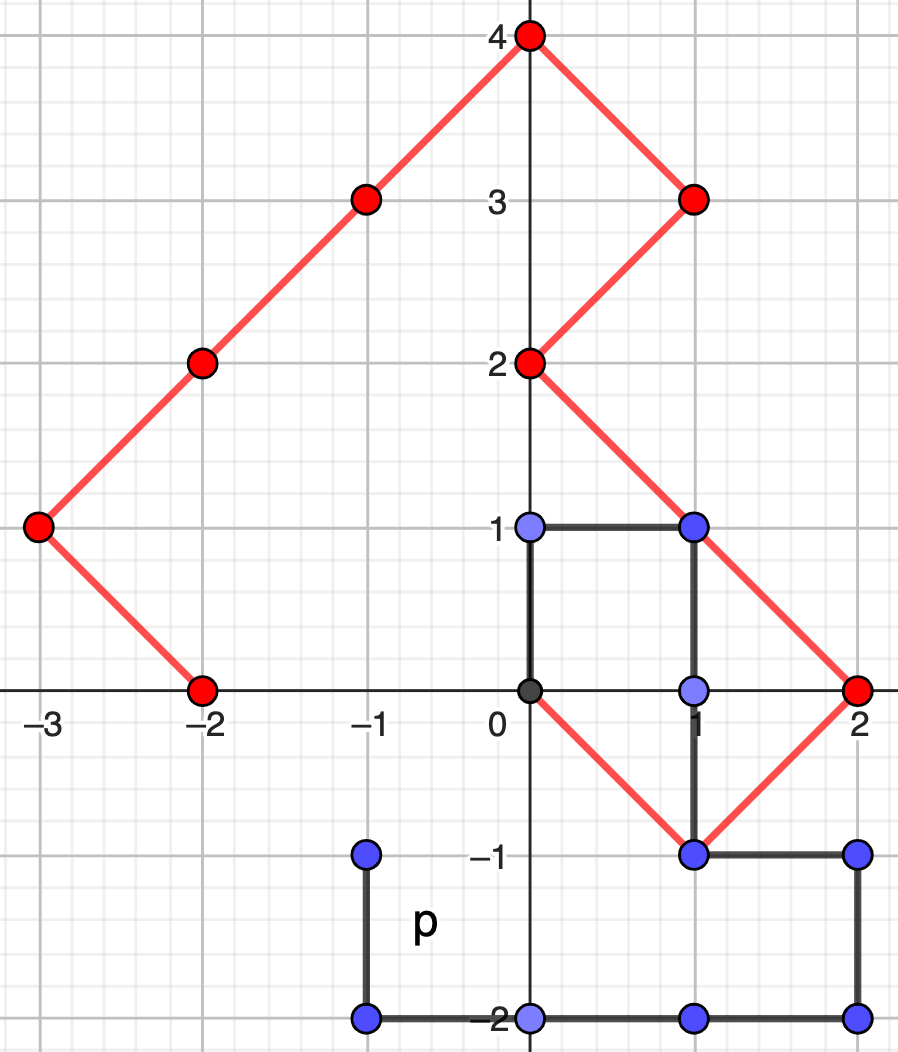
\includegraphics[height=5cm]{figures/marche_Z2.png}
        }
%-----------------------
    \item Les variables $U_n$ et $V_n$ sont-elles indépendantes ?
%-----------------------
        \cor{
            Oui car \\
            $\bbP(U_n=V_n=1)=\bbP(X_n=1,Y_n=0)=1/4=\bbP(U_n=1)\bbP(V_n=1)$,\\
            $\bbP(U_n=V_n=-1)=\bbP(X_n=-1,Y_n=0)=1/4=\bbP(U_n=-1)\bbP(V_n=-1)$,\\
            $\bbP(U_n=1,V_n=-1)=\bbP(X_n=0,Y_n=1)=1/4=\bbP(U_n=1)\bbP(V_n=-1)$,\\
            $\bbP(U_n=-1,V_n=1)=\bbP(X_n=0,Y_n=-1)=1/4=\bbP(U_n=-1)\bbP(V_n=1)$.
        }
%-----------------------
    \item Calculer $\bbP(S_n=(0,0))$. 
%-----------------------
        \cor{
            \begin{align*}
                (S_n=(0,0))&= \Big(\sum_{k=1}^n X_k=0, \sum_{k=1}^n Y_k=0\Big)\\
                &= \Big(\sum_{k=1}^n X_k+\sum_{k=1}^n Y_k=0, \sum_{k=1}^n X_k-\sum_{k=1}^n Y_k=0\Big)\\
                &= \Big(\sum_{k=1}^n U_k=0, \sum_{k=1}^n V_k=0\Big)
            \end{align*}
            Or les suites $(U_n)$ et $(V_n)$ sont indépendantes, donc\\
            $\bbP(S_n=(0,0))=\bbP(S_n^U=0)\bbP(S_n^V=0)$\\
            où $(S_n^U)$ et $(S_n^V)$ sont des marches aléatoires simples symétriques  en dimension $1$, issues de $0$, avec incréments $(U_k)$ et $(V_k)$ respectivement. D'après le cours, cette probabilité est nulle si $n$ est impair et \\
            $\bbP(S_{2n}=(0,0))=\bbP(S_{2n}^U=0)\bbP(S_{2n}^V=0)=\Big(\frac{1}{4^n}C_{2n}^n\Big)^2$.
            En suivant un raisonnement analogue à celui du cours, on peut montrer que la marche aléatoire en dimension $2$ est encore récurrente (ce qui ne sera plus vrai à partir de la dimension $3$).
        }
%-----------------------
\end{enumerate}
\end{exo}
%=========================
\end{document}

